Throughout all this document, we will use a lot of results from algebra. This
chapter is here to sum up these results and try to maintain the illusion that
this thesis is self-contained. Our references for standard results in algebra are
~\cite{Lang04} or~\cite{Perrin96}.
The reader familiar with the notions of finite
fields, algebraric function fields, complexity model may very well skip this
chapter.
\minitoc
 
% TODO: picture

% TODO
% ====
%
% - Add a subsection on classic subroutines, e.g. definition of the function
%   M(·) (the cost of the multiplication of polynomials), probably also modular
%   composition, maybe transposition principle?
%
% - Finish the different sections

\section{Finite fields}

Finite fields are ubiquitous in cryptography and coding theory, probably because
their field structure, a rigid one, allows to understand how they work, and
their finiteness makes them easier to represent on a computer. They are also
everywhere in this thesis, and are probably on almost every paper I
wrote on during these last three years. They are quite important. A detailed
book about finite fields is~\cite{LN97}.

\subsection{Finite field structure}

A \emph{finite field} is a field $\K$ whose cardinality is finite. The first
examples of finite fields are the rings 
\[
  \mathbb{Z}/p\mathbb{Z}
\]
with $p\in\mathbb{N}$ a prime number. More generally, we denote by
$\mathbb{F}_{q}$ the finite field with $q$ elements. The cardinality of a finite
field is very well understood.
\begin{prop}
 There exists a unique (up to isomorphism) finite field of cardinality $q = p^l$
 for earch prime number $p\in\mathbb{N}$ and integer $l\geq1$.
\end{prop}
Let $q=p^l$ a prime power, there are several ways of representing
\emph{the} finite field with $q$ elements, but the one that we will almost
always have in mind is the following.

\begin{prop}
Let $P\in\mathbb{F}_p[x]$ be an
irreducible polynomial of degree $l$ with coefficients in $\mathbb{F}_p$. Then
\[
  \mathbb{F}_p[x]/(P(x))
\]
is a finite field with $q = p^l$ elements.
\end{prop}
We often write
\[
  \mathbb{F}_q \cong \mathbb{F}_{p}[x]/(P(x))\cong \mathbb{F}_p(\alpha)
\]
in order to say that we work with a finite field of $q$ elements, represented by
the quotient $\mathbb{F}_{p}[x]/(P(X))$, and where the projection of $x$ in the
quotient is denoted by $\alpha=\bar x$.

\subsection{Subfields and field extensions}

The finite field $\mathbb{F}_{p^l}$ is a
field extension of $\mathbb{F}_{p}$ of dimension $l$, \ie it is a
$\mathbb{F}_{p}$-vector space of dimension $l$. When dealing with the vector
space structure of $\mathbb{F}_{p^l}=\mathbb{F}_{p}(\alpha)$, we almost always choose to work with the
cannonical basis 
\[
  1, \alpha, \alpha^2, \dots, \alpha^{l-1}.
\]
Other interesting types of bases exist, such as for example normal
bases~\cite{Gao93}, but we always precise the basis when it is not clear from
the context.
Given $q=p^m$ a prime power and
$l\in\mathbb{N}$ an integer, we also write 
\[
  \mathbb{F}_{q^l}
\]
the field with $q^l = p^{ml}$ elements. We have
\[
  \mathbb{F}_{q^l}\cong\mathbb{F}_{p^{lm}},
\]
but the difference is that we see $\mathbb{F}_{q^l}$ as an extension of
$\mathbb{F}_{q}$ of dimension $l$, and not as an extension of the prime field
$\mathbb{F}_p$. Again, we usually think that our field $\mathbb{F}_{q^l}$ is
represented as
\[
  \mathbb{F}_{q^l}=\mathbb{F}_q[x]/(P(x)),
\]
where $P(x)\in\mathbb{F}_{q}[x]$ is an irreducible polynomial of degree $l$ with
coefficients in the base field $\mathbb{F}_q$. The subfields of
$\mathbb{F}_{q^l}$ are also well understood.
\begin{prop}
  \label{prop:subfields}
  Let $q=p^m$ be a prime power and $l\in\mathbb{N}$ an integer. Then there is
  an extension $\mathbb{F}_{q^m}$ of $\mathbb{F}_q$ of degree $m$ 
  included in $\mathbb{F}_{q^l}$
  \[
    \mathbb{F}_{q^m}\subset\mathbb{F}_{q^l}
  \]
  if and only if $m$ divides
  $l$. The elements in this subfield of $\mathbb{F}_{q^l}$ are the roots of the
  polynomial
  \[
    x^{q^m}-x
  \]
  in $\mathbb{F}_{q^l}$.
\end{prop}
Figure~\ref{fig:F12} describes the subfields of $\mathbb{F}_{12}$, as an
illustration of Proposition~\ref{prop:subfields}.
\begin{figure}
  \centering
  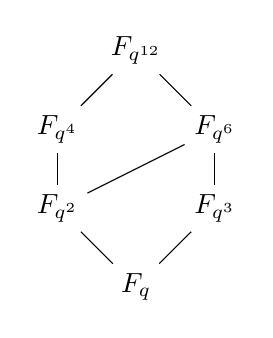
\begin{tikzpicture}
    \node (1) at (0,0) {$\mathbb{F}_{q}$}; 
    \node (2) at (-1,1) {$\mathbb{F}_{q^2}$}; 
    \node (3) at (1,1) {$\mathbb{F}_{q^3}$}; 
    \node (4) at (-1,2) {$\mathbb{F}_{q^4}$}; 
    \node (6) at (1,2) {$\mathbb{F}_{q^6}$}; 
    \node (12) at (0,3) {$\mathbb{F}_{q^{12}}$}; 
    \draw (1) -- (2);
    \draw (1) -- (3);
    \draw (2) -- (4);
    \draw (2) -- (6);
    \draw (3) -- (6);
    \draw (6) -- (12);
    \draw (4) -- (12);
  \end{tikzpicture}
  \caption{The subfields of $\mathbb{F}_{12}$. Two fields are linked if one is a
subfield of the other.}
  \label{fig:F12}
\end{figure}
The $\mathbb{F}_q$-automorphisms of the extension $\mathbb{F}_{q^l}$ are given
by the following result.
\begin{prop}
  Let $q=p^m$ be a prime power and $l\in\mathbb{N}$ an integer.
  The group of $\mathbb{F}_q$-automorphisms of $\mathbb{F}_{q^l}$ is a cyclic
  group of order $l$ generated by
  \[
    \sigma : t\mapsto t^q.
  \]  
\end{prop}
Let $u\in\mathbb{F}_{q^l}$, the conjugates of $u$ are the elements
\[
  \sigma(u), \sigma^2(u), \dots, \sigma^{l-1}(u)
\]
and the orbit of $u$ is the set
\[
  \left\{ u, \sigma(u), \dots, \sigma^{l-1} \right\}.
\]
This orbit might have any length $m$ dividing $l$. The orbit of $u$ is of length
$m$ if and only if $u$ is in a subfield $\mathbb{F}_{q^m}$ of
$\mathbb{F}_{q^l}$. We also sometimes write
\[
  u^\sigma = \sigma(u).
\]
Two maps, defined with the conjugates of a given element,
will play a very important role, the \emph{trace} and the \emph{norm}.
\begin{defi}[Trace and norm]
  Let $q$ a prime power and 
  \[
    \mathbb{F}_{q^l}/\mathbb{F}_q
  \]
  an extension of degree $l$, let $G$ be the group of
  $\mathbb{F}_q$-automorphisms of $\mathbb{F}_{q^l}$, and let
  $u\in\mathbb{F}_{q^l}$. Then the \emph{trace} of $u$ is
  \[
    \tr_{\mathbb{F}_{q^l}/\mathbb{F}_q}(u) = \sum_{\sigma\in G}u^\sigma
  \]
  and the \emph{norm} of $u$ is
  \[
    N_{\mathbb{F}_{q^l}/\mathbb{F}_q}(u)=\prod_{\sigma\in G}u^\sigma.
  \]
\end{defi}
We may only write $\tr$ or $N$ when the extension considered is clear from the
context. The trace over the field $\mathbb{F}_{q}$ is a $\mathbb{F}_{q}$-linear
map, and the norm is a multiplicative map, they are also both \emph{transitive},
as described in the next proposition.
\begin{prop}
  Let $q\in\mathbb{N}$ a prime power and $a\,|\,b\,|\,c$ three integers, giving
  the tower of extensions that follows.
  \begin{center}
  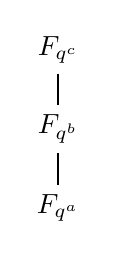
\begin{tikzpicture}
    \node (a) at (0,0) {$\mathbb{F}_{q^a}$}; 
    \node (b) at (0,1) {$\mathbb{F}_{q^b}$}; 
    \node (c) at (0,2) {$\mathbb{F}_{q^c}$}; 
    \draw (a) -- (b);
    \draw (b) -- (c);
  \end{tikzpicture}
  \end{center}
  Let $u\in\mathbb{F}_{q^c}$, then
  \[
    \tr_{\mathbb{F}_{q^c}/\mathbb{F}_{q^a}}(u) =
    \tr_{\mathbb{F}_{q^b}/\mathbb{F}_{q^a}}(\tr_{\mathbb{F}_{q^c}/\mathbb{F}_{q^b}}(u))
  \]
  and
  \[
    N_{\mathbb{F}_{q^c}/\mathbb{F}_{q^a}}(u) =
    N_{\mathbb{F}_{q^b}/\mathbb{F}_{q^a}}(N_{\mathbb{F}_{q^c}/\mathbb{F}_{q^b}}(u)).
  \]
\end{prop}
Finally, the map
\[
  (x, y)\mapsto\tr(xy)
\]
is a non-degenerate bilinear map that we will also sometimes write as
\[
  \ps{x}{y} = \tr(xy).
\]
%
%\subsection{Kummer extensions}
%
%Kummer extensions are a particular kind of extension, they play a special role in
%our construction of lattices of extension presented in
%Chapter~\ref{chap:lattice}. We follow the presentation of~\cite{Lang04}.

\section{Algebraic function fields}
\label{sec:algebraic-function-fields}

% Contents
% ========
%
% - algebraic function field
% - place
% - degree of a place
% - divisor
% - big theorems
% - definition of the genus ?

Together with algebraic curves, algebraic function fields are a way of
describing the algorithms of Chapters~\ref{chap:bilinear}
and~\ref{chap:hypersymmetric}. In this document, we choose to use the algebraic
function field point of view. The function fields we need are constructed
on top of finite fields, so we present the theory with that context in mind. For
this section, our reference is~\cite{Stichtenoth09}. In all the section, $\K$ is
a finite field of characteristic $p$.

\subsection{Places}

Let us first define what an algebraic function field is, together with important
notions leading to the definition of \emph{places}.
\begin{defi}[Algebraic function field]
  An \emph{algebraic function field} $F$ of one variable over $\K$ is an
  extension field 
  \[
    F/\K
  \]
  such that $F$ is a finite algebraic extension of
  $\K(x)$ for some element $x\in F$ which is transcendental over $\K$.
\end{defi}
From now on, the notation $F$ will represent an algebraic function field over
$\K$.
\begin{defi}[Valuation ring]
  A \emph{valuation ring} $\vr$ of the function field $F/\K$ is a ring 
  \[
    \vr \subset F
  \]
  with the following properties
  \begin{enumerate}
    \item $\K\subsetneq\vr\subsetneq F$;
    \item for all $z\in F$, we have $z\in\vr$ or $z^{-1}\in\vr$.
  \end{enumerate}
\end{defi}
Valuation rings $\vr$ are local rings, \ie they have a unique maximal ideal that is
given by 
\[
  P = \vr\setminus\vr^\times
\]
where $\vr^\times$ is the group of units of the ring $\vr$.
\begin{defi}[Place]
  A \emph{place} $P$ of $F$ is the maximal ideal of some valuation ring $\vr$ of $F$.
\end{defi}

% Note
% ====
%
% Maybe a word about the equivalence of the notions of places, discrete valuation
% and valuation ring could be nice here, just a proposition without a proof or
% even a remark not too formal, we'll see.

We let $\mathbb{P}_F$ be the set of places of $F$. If $P\in\mathbb{P}_F$ is a
place of $F$, we denote by $\vr_P$ the corresponding valuation ring. Since $P$
is a maximal ideal of $\vr$, we also know that the quotient ring
\[
  F_P = \vr_P/P
\]
is a field. We call this field $F_P$ the residue class field of $P$.
\begin{defi}[Residue class map]
Let $P\in\mathbb{P}_F$ be a place of $F$. For $x\in F$, we let 
\[
  x(P)
\]
be the residue class of $x$ modulo $P$. If $x\notin P$, we define $x(P)=\infty$.
The map from $F$ to $F_P\cup\left\{ \infty \right\}$
\[
  x\mapsto x(P)
\]
is called the \emph{residue class map}.
\end{defi}
\begin{defi}[Degree of a place]
  Let $P\in\mathbb{P}_F$ a place of $F$. The residue class field $F_P$ is a
  finite extension of $\K$ and we call
  \[
    \deg P = \left[ F_P\,:\,\K \right]
  \]
  the \emph{degree} of $P$.
\end{defi}

\subsection{Divisors}

Now that we now what places are, we can define divisors. In this section, we
keep the notation of last section: we let $F$ be an algebraic function field
over a finite field $\K$ of characteristic $p$.
\begin{defi}[Divisor]
  The \emph{divisor group} $\Div(F)$ of $F$ is defined as the free abelian group generated
  with the places of $F$. The elements of $\Div(F)$ are called the
  \emph{divisors} of $F$. In other words, a divisor is a formal sum
  \[
    D = \sum_{P\in\mathbb{P}_F} n_P\cdot P
  \]
  with $n_P\in\mathbb{Z}$ and $n_P=0$ for all but finitely many places $P$.
  We define the \emph{support} of $D$ as
  \[
    \supp D = \left\{ P\in\mathbb{P}_F\,|\,n_P\neq 0 \right\}.
  \]
\end{defi}


\section{Complexity models}
\label{sec:complexity-models}

In algorithmic, it is of central interest to understand how our algorithms
\emph{scale}, \ie to understand how they perform if the size of the input is
getting larger and larger. Complexity theory studies this phenomenon and give us models
of computation in order to quantify the behaviour of our algorithms. Depending
on the situation, not all models are relevant, and one has to balance between
the concreteness of a model and its ease to use. An extreme viewpoint is to
specify an operating system with a compiled programming language and to compare
the running time or the memory requirements between algorithms. The advantage of
such a model is that it is very concrete, but it is also its main disadvantage
because it makes the model hard to use. Thus, there exist other models of
\emph{idealized} computer, such as Turing machines~\cite{Papadimitriou03},
random access machines, or the algebraic complexity model.
We use the latter, that we present in more details in the next section.

\subsection{Algebraic complexity}

This model is widely presented in~\cite{BCS13}, we only give a brief
presentation of the subject. This model assumes that we use an abstract computer
that is able to perform operation in some base field $\K$ at a constant, unit
cost. We also assume that accessing the memory of the computer is free.
Algebraic complexity is especially useful with algorithms dealing with
algebraic structures. This is very handy for us, since
we usually work with algebras
\[
  (\A, +, \times, \cdot)
\]
over some base field $\K$. As an example, with this model, the complexity of an
addition in the extension field
\[
  \mathbb{F}_4 = \mathbb{F}_2[T]/(T^2+T+1) = \mathbb{F}_2(x)
\]
where $x=\bar T$, if elements are represented in the basis $\left\{ 1, x
\right\}$, is $2$, because we only need $2$ additions in $\mathbb{F}_2$ to
perform an addition in $\mathbb{F}_4$. Indeed, if
\[
  a = a_0 + a_1x\in\mathbb{F}_4
\]
and
\[
  b = b_0 + b_1x\in\mathbb{F}_4,
\]
we have
\[
  a+b = (a_0+b_0)+(a_1+b_1)x.
\]
In the case of a multiplication, we have
\[
  ab = (a_0b_0+a_1b_1) + (a_0b_1+a_1b_0)x,
\]
so the complexity of a multiplication in $\mathbb{F}_4$ (at least with this
formula) is $6$, because we need
$4$ multiplications and $2$ additions in $\mathbb{F}_2$. In the context of
finite fields, it makes sense to consider that the cost of an operation is
independent of the operands, because the elements have a fixed size; but this is
no longer the case in other rings, for example in $\mathbb{Z}$, $\mathbb{Q}$,
$\mathbb{R}$, or $\mathbb{C}$. We could also argue that the different operations
in $\K$ should not have the same cost, we thus present an other manner of
computing the complexity of an algorithm, that is called \emph{bilinear
complexity}, in Chapter~\ref{chap:bilinear}.

\subsection{Landau notations}

In order to describe the asymptotic behaviour of an algorithm, we use the
classical \emph{big O} and \emph{little o} notations $O$ and $o$. Let $f:\mathbb{R}\to\mathbb{R}$ and
$g:\mathbb{R}\to\mathbb{R}$ be two functions, we write
\[
  f(x) = O(g(x))
\]
if there exist $M\in\mathbb{R}$ and $C>0$ such that
\[
  \forall x\geq M,\,|f(x)|\leq Cg(x).
\]
and we write
\[
  f(x)=o(g(x))
\]
if there exist $M\in\mathbb{R}$ and $\varepsilon:\mathbb{R}\to\mathbb{R}$, a
function with $\varepsilon(x)\to 0$ when $x\to\infty$, such
that
\[
  \forall x\geq M,\,|f(x)|\leq \varepsilon(x)g(x).
\]
We say that $f$ is equivalent to $g$ and we write
\[
  f(x)\sim g(x)
\]
if 
\[
 f(x)-g(x) = o(g(x))
\]
when $x\to\infty$. Finally, we also use the \emph{soft O} notation $\tilde{O}$ to neglect
logarithmic factors in the big O notation, we write
\[
  f(x) = \tilde{O}(g(x))
\]
if there exist some $k$ with $f(x) = O(g(x)\log^k(g(x)))$.

